\section{Desarrollo}

\subsection{Fuente $S$}

\par Definiremos una fuente de memoria nula $S$ en base a los frames de capa de enlace capturados. 
La fuente consiste en dos mensajes: un frame fue transmitido de forma \textit{broadcast}, o éste fue transmitido de forma \textit{unicast}.

\subsection{Elección de la fuente $S_1$}

\par Definiremos una fuente de memoria nula $S_1$ en base a las Direcciones IP de los paquetes ARP. 
Deberemos tomar diversas decisiones para definirla correctamente para poder distinguir los nodos apropiados.

\par En primer lugar: debemos elegir si tomar los paquetes \textit{who-has}, \textit{is-at}, o ambos.
En la mayoría de los casos, un \textit{who-has} será respondido por exactamente un \textit{is-at} correspondiente, a menos que el receptor deseado no pueda recibir el paquete o emitir la respuesta, o que haya dos dispositivos con una misma MAC address que intenten responder a la vez.
Por ende, la información del \textit{is-at} será redundante con la del \textit{who-has}, a menos que se produzca un error (lo que, de tomar ambos, agregaría errores a las mediciones).

\par Consecuentemente, tomaremos sólo uno.
Ya que el \textit{who-has} se transmite de forma \textit{broadcast}, mientras que el \textit{is-at}, de forma \textit{unicast}\footnote{Si bien realizaremos las mediciones en modo promiscuo, la presencia de \textit{switches} puede evitar que veamos este tipo de paquetes si no están destinados a nuestro dispositivo, lo que generaría aún más errores en las mediciones.}, tomaremos el primero.

\par En segundo lugar, debemos decidir si emplear el origen del \textit{who-has}, su destino, o ambos como el mensaje de la fuente.
Esta decisión no la tomaremos de antemano, sino que observaremos los grafos resultantes de los experimentos y en base a ellos decidiremos cuál es la opción más acertada.

\par En último lugar, debemos decidir si permitir mensajes repetidos\footnote{Es decir, si considerar repetidas veces múltiples paquetes ARP con igual origen y destino.}. 
Si bien esto no es ilógico desde el punto de vista del modelo de fuente de memoria nula planteado, los paquetes ARP repetidos no deberían ser necesarios: una vez que se envía un \textit{who-has} por una cierta dirección IP y éste es respondido por un \textit{is-at}, la relación entre esta dirección y la MAC address provista debería persistirse en una tabla del emisor; paquetes repetidos podrían ser síntomas de que el \textit{who-has} original no tuvo respuesta, por lo que otros posteriores fueron requeridos.

\par Creemos que por esta razón no deberíamos considerar paquetes repetidos, pero de todas formas juzgaremos ambos procedimientos en base a los resultados de los experimentos.

\par Los grafos que emplearemos para representar la red subyacente de mensajes ARP serán independientes de las elecciones que tomemos respecto de la fuente.
En particular, éstos consistirán en digrafos con loops\footnote{Como mencionamos en la Introducción, en un \textit{gratuitous ARP}, $\text{\textit{Sender's Protocol Address}} = \text{\textit{Target Protocol Address}}$. Para poder observar este fenómeno en el grafo, permitiremos loops.}, donde hay un eje de un nodo a otro si el primero emite un \textit{who-has} preguntando por la Dirección IP del segundo.
 
\newpage
\subsection{Experimento 1: red inalámbrica de los laboratorios del DC}
\par Para este experimento evaluamos la red inalámbrica de los laboratorios del DC.

\subsubsection{Fuente $S$}

\par A continuación podemos ver la fuente $S$ propuesta, modelada con los resultados del experimento: \\

\begin{tabular}{ | c | c | c |}
    \hline
    Mensaje & Probabilidad & Información [bits] \\
    \hline
    \textit{Unicast} & 0.773 & 0.371 \\
    \hline
    \textit{Broadcast} & 0.227 & 2.141 \\
    \hline
\end{tabular} \\

\par Entropía de la fuente: 0.772 bits. Entropía máxima: 1 bit.

\par Observamos que la entropía de la fuente es menor que la máxima, ya que las transmisiones \textit{unicast} son casi 3 veces más probables que las \textit{broadcast}.
Esto nos provee una cota inferior para el \textit{overhead} impuesto por los protocolos de control: al menos 22.7\% de los frames no transmiten datos.

\par Ya que no poseemos una idea del comportamiento esperado de esta fuente, no podemos realizar un análisis más detallado sólo a partir de esta fuente.
Por ende, lo profundizaremos recién en la sección del siguiente experimento, comparando con los resultados obtenidos de esa red.
%vemos que la entropía y la probabilidad de los frames \textit{broadcast} son significativamente mayores para la fuente $S$ en el experimento 2.

%\par Podemos ver, comparando la estructura de ambas redes (figuras \ref{ARPDC-sinColapsar} y \ref{ARPTrab-sinColapsar}, respectivamente), que la de este experimento es más fragmentaria, mientras que la del 2 posee un mucho mayor grado de interconexión.

\subsubsection{Estructura de la red en base a los paquetes ARP}

\par En las figuras \ref{ARPDC-sinColapsar} y \ref{ARPDC} se pueden ver los grafos\footnote{Ambos grafos representan la misma red. Sin embargo, el tamaño del grafo \ref{ARPDC-sinColapsar} puede dificultar un análisis detallado, por lo que en la figura \ref{ARPDC} colapsamos ciertos nodos con iguales vecinos (que se muestran en rojo). Mantuvimos el grafo original ya que una mirada rápida ofrece más información concerniente a la topología de la red.} de la red subyacente de mensajes ARP.

\begin{figure*}[ht]
    \centering
    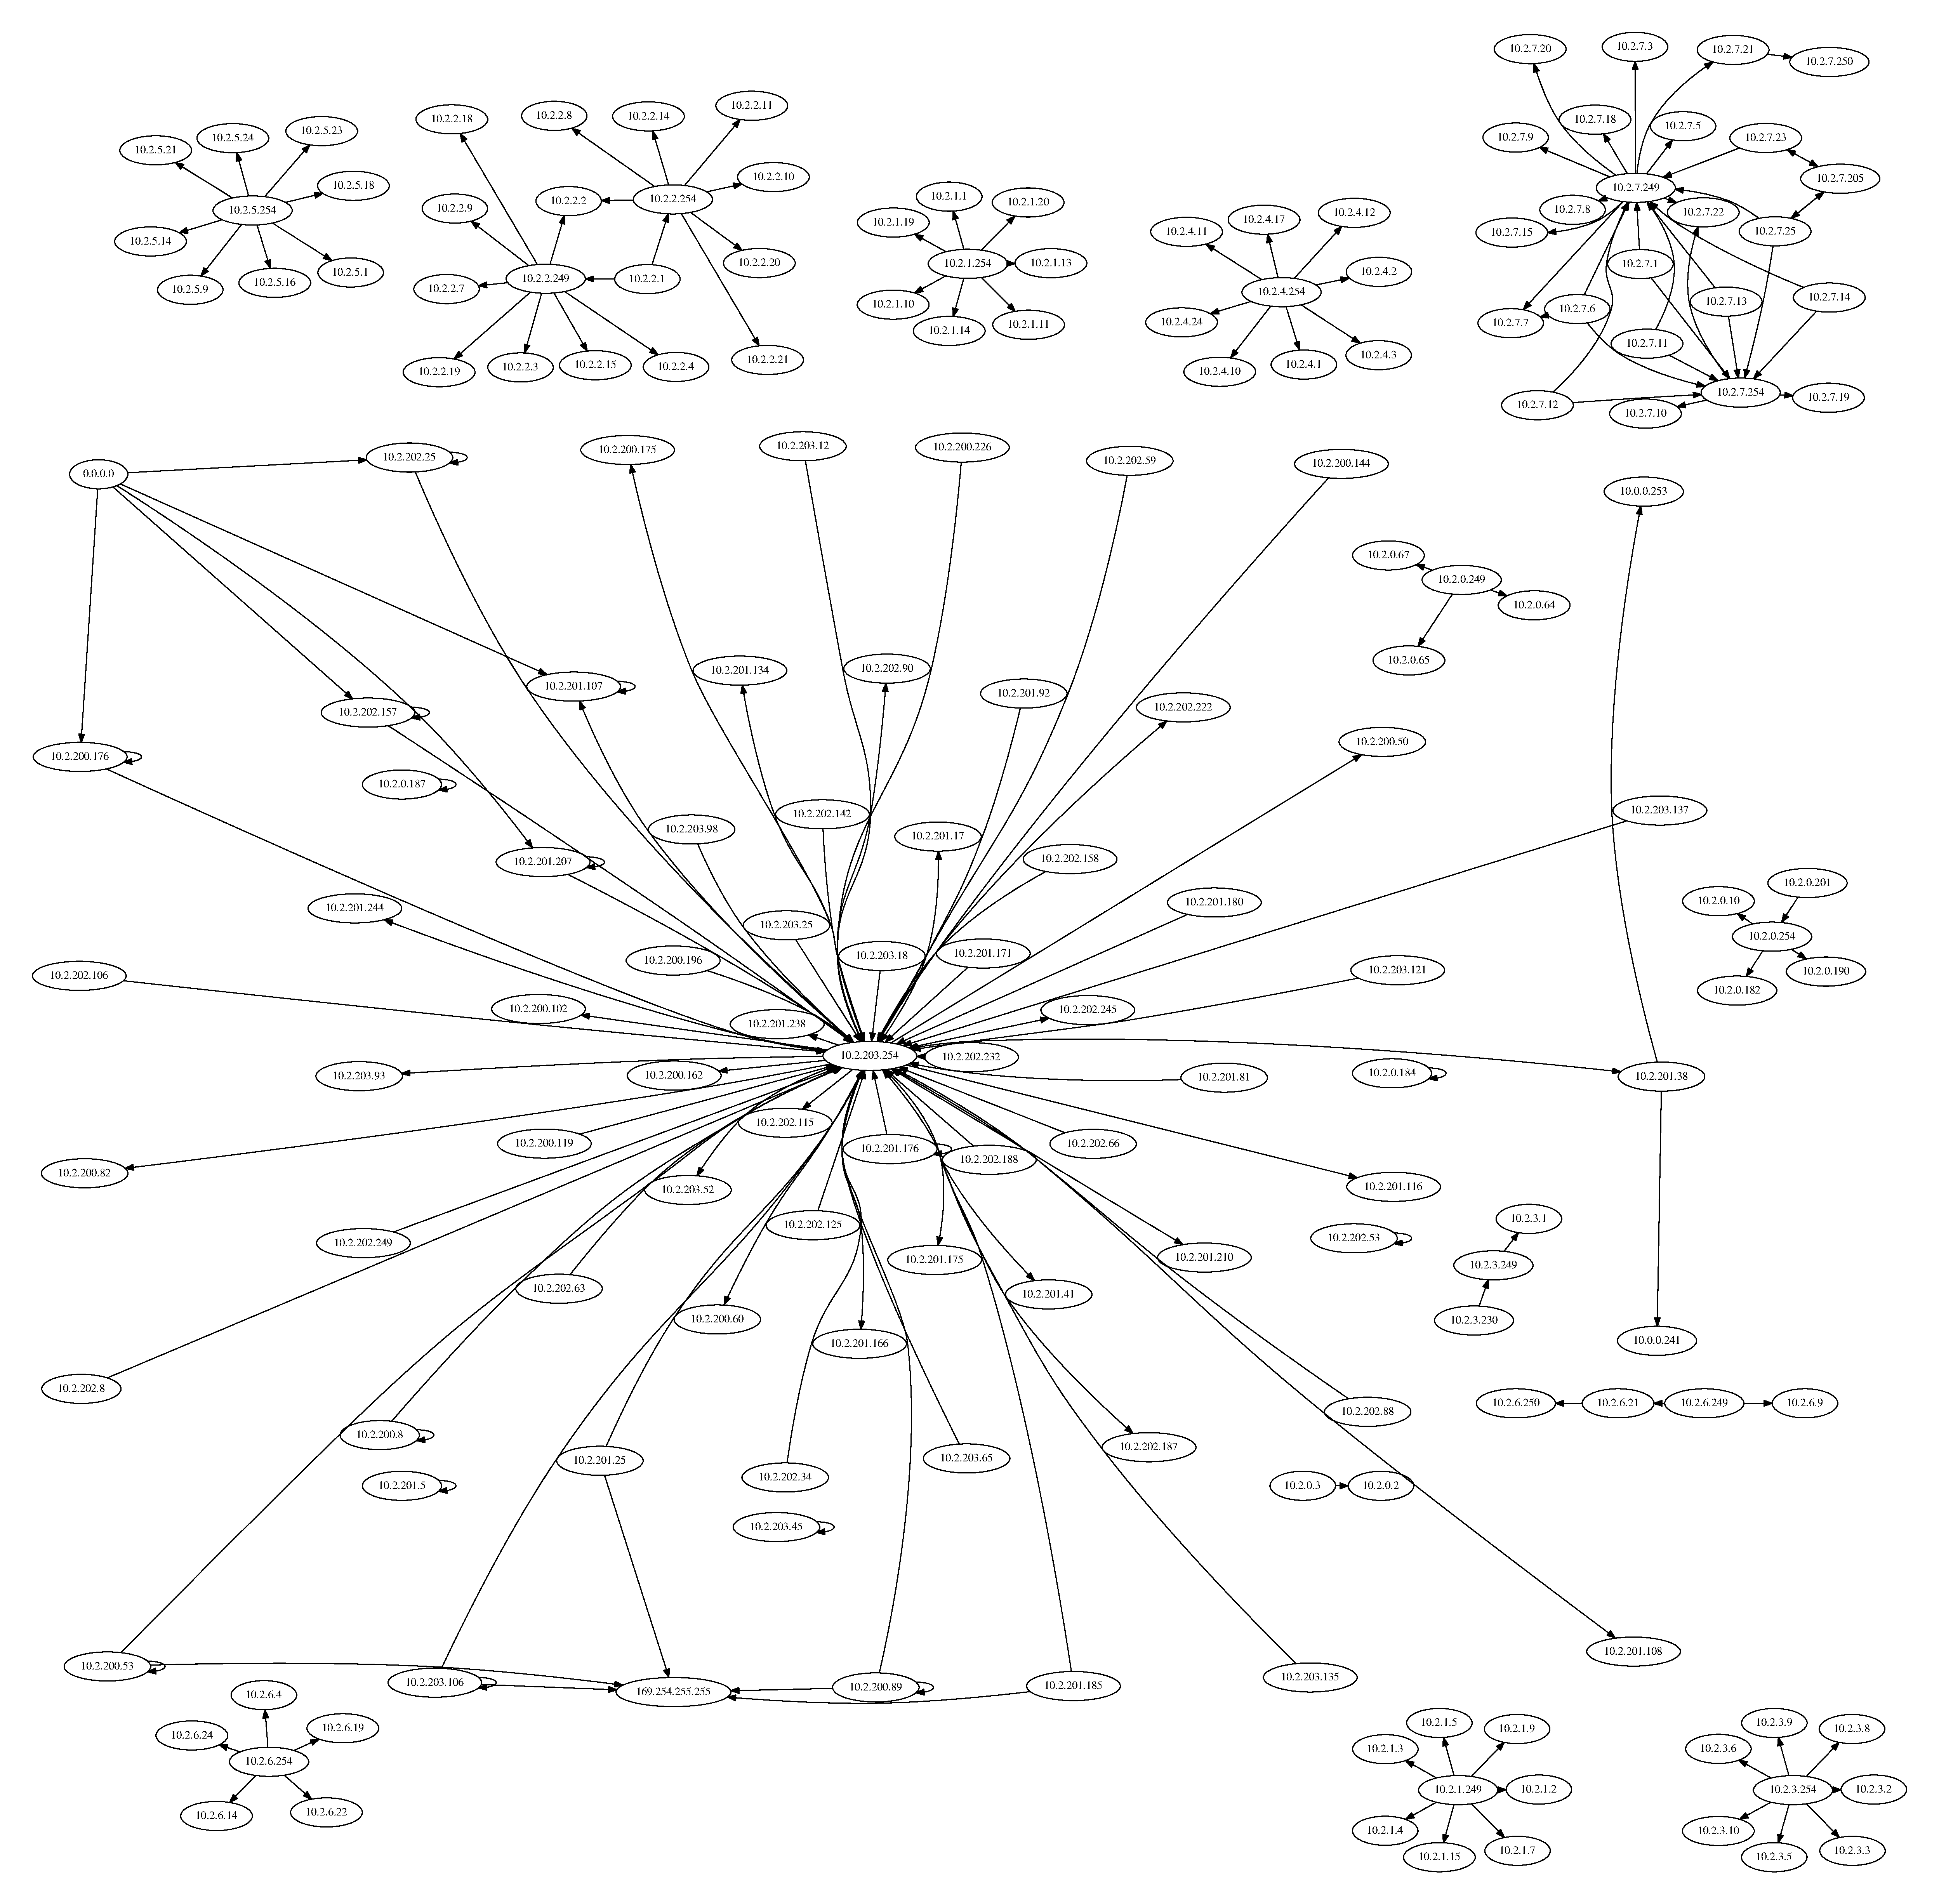
\includegraphics[width=0.9\textwidth]{figuras/ciudad_10_grafoSinColapsar.pdf}
    \caption{Grafo de la red subyacente de mensajes ARP, sin colapsar nodos .}\label{ARPDC-sinColapsar}
\end{figure*}

\begin{figure*}[ht]
    \centering
    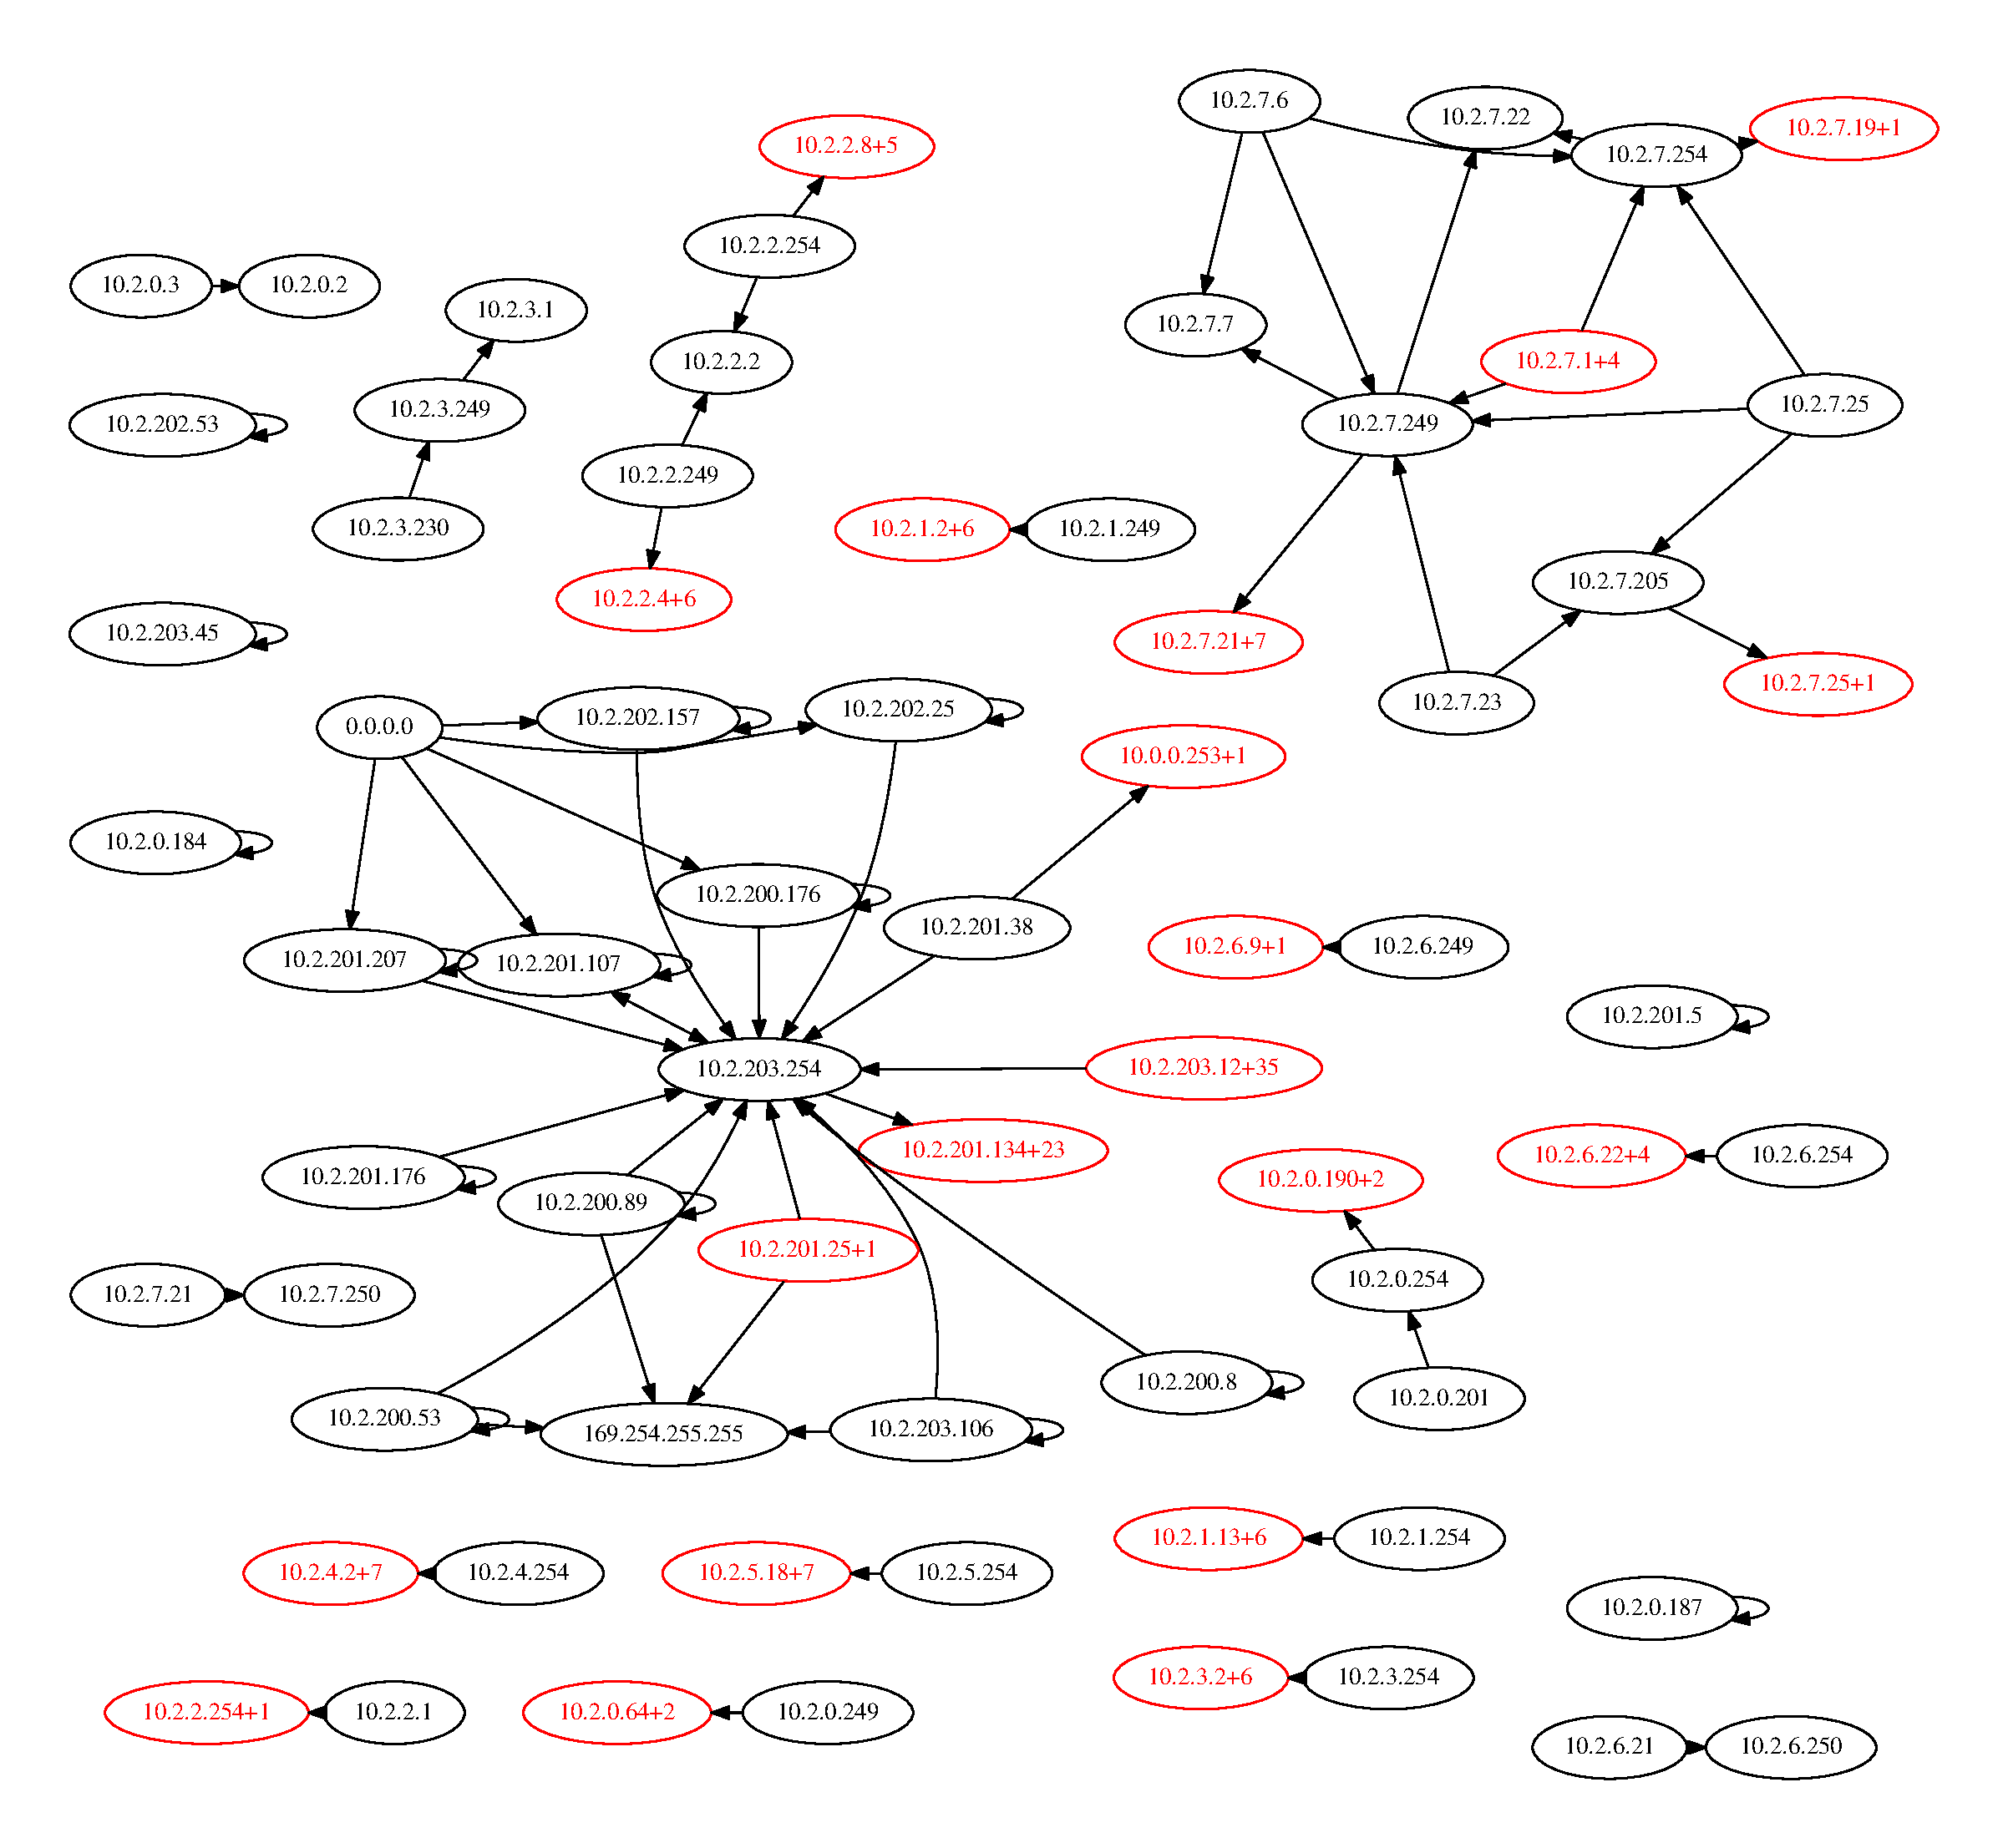
\includegraphics[width=0.9\textwidth]{figuras/ciudad_10_grafo.pdf}
    \caption{Grafo de la red subyacente de mensajes ARP, colapsando nodos.}\label{ARPDC}
\end{figure*}

\par Las direcciones IP de la red son de la forma 10.2.X.Y, con una sola excepción que mencionaremos más adelante.
Éstas son direcciones IP privadas\footnote{Todo el rango 10.0.0.0-10.255.255.255 es privado.}.

\par La red se presenta altamente fragmentada; el grafo posee múltiples componentes conexas.
Adicionalmente, vemos repetido un patrón entre varias de estas componentes: un nodo central, con una dirección IP de la forma 10.2.X.254 o 10.2.X.249, que envía paquetes a múltiples hojas\footnote{Se presenta una estructura de estrella, o cercana.}.
Esta estructura es consistente con el comportamiento esperado de Default Gateways. 

\par Hay un nodo claramente destacado en la red, el de dirección IP 10.2.203.254, que tanto envía como recibe paquetes de un gran número de hojas.

\par Se advierten diversas anomalías: en primer lugar, loops en el grafo, que como mencionamos previamente, se deben a \textit{gratuitous ARPs}; en segundo lugar, la dirección 0.0.0.0 se hace presente en el grafo, siempre como origen, lo que ejemplifica \textit{ARP probing}; finalmente, una única IP que no comienza con 10.2, la 169.254.255.255.
El rango 169.254.0.0-169.254.255.255 está reservado; se asigna cuando un dispositivo no tiene IP estática, y el protocolo dinámico\footnote{DHCP siendo actualmente el más común.} utilizado falla.

\subsubsection{Fuente $S_1$}

\par En la tabla \ref{tab1SinRSinA} podemos ver la información de ciertos\footnote{La alta cantidad de nodos dificulta seriamente la presentación de estos resultados, tanto en forma de gráficos como de tablas.
En las siguientes tablas listaremos todos los nodos distinguidos, y los nodos que, en base a ciertos criterios, nos parecieron destacados pero la fuente no distinguió.} mensajes de la fuente $S_1$, sin paquetes repetidos y tomando sólo el \textit{Sender's Protocol Address} de los paquetes.

\par La entropía de la fuente es de 5.61 bits, siendo la máxima 32 bits. 

\begin{table}[t]
    \centering
    \begin{tabular}{ | c | c | c | l |}
        \hline
        Mensaje & Información [bits] & Distinguido?\\
        \hline
        10.2.3.249 & 7.58 & No \\ %
        \hline
        10.2.202.249 & 7.58 & No \\ %
        \hline
        10.2.6.249 & 6.58 & No \\ %
        \hline
        10.2.7.254 & 6.00 & No \\
        \hline
        10.2.0.254 & 6.00 & No \\
        \hline
        10.2.0.249 & 6.00 & No \\
        \hline
        10.2.6.254 & 5.26 & Sí \\
        \hline
        10.2.1.254 & 4.78 & Sí \\
        \hline
        10.2.1.249 & 4.78 & Sí \\
        \hline
        10.2.3.254 & 4.78 & Sí \\
        \hline
        10.2.2.254 & 4.78 & Sí \\
        \hline
        10.2.2.249 & 4.58 & Sí \\
        \hline
        10.2.4.254 & 4.58 & Sí \\
        \hline
        10.2.5.254 & 4.58 & Sí \\
        \hline
        10.2.7.249 & 4.26 & Sí \\
        \hline
        10.2.203.254 & 2.94 & Sí \\
        \hline
    \end{tabular} 
    \caption{Información de los nodos de la fuente $S_1$, sin tomar paquetes repetidos y considerando como mensaje la ocurrencia de una IP en el campo \textit{Sender's Protocol Address} de un paquete ARP \textit{who-has}.}
    \label{tab1SinRSinA}
\end{table} 

\par Vemos que no se producen falsos positivos: todos los nodos que la fuente distingue son los que destacamos previamente, con direcciones IP de la forma 10.2.X.249 o 10.2.X.254.
Sin embargo, vemos ciertos potenciales falsos negativos.

\par Los tres primeros, es decir el 3.249, el 202.249 y el 6.249\footnote{Obviando de las direcciones el 10.2. inicial.}, si bien sus IPs son de la forma destacada, no parecen exhibir el comportamiento de los otros\footnote{En el grafo no se presentan en el centro de una estructura de estrella o similar.} ni actuar como Default Gateways.
Por ende, concluimos que no clasificarlos como distinguidos no es una falencia de la fuente.

\par Sin embargo los tres restantes, el 7.254, el 0.249 y el 0.254, presentan el comportamiento mencionado y exhiben la estructura de estrella, pero no son clasificados como distinguidos.
En el caso del 0.249, esto se debe a que no tiene suficientes vecinos, por lo que su información es relativamente baja; es posible que esta falencia pueda ser subsanada al considerar paquetes repetidos.
Por otro lado, el 0.254 y el 7.254, tienen más vecinos pero varios de éstos presentan ejes en el otro sentido que el aceptado por la fuente\footnote{Es decir, este nodo es el destino de varios paquetes ARP, no el origen.}; es posible que este error sea resuelto aceptando ejes en ambas direcciones.

\par En la tabla \ref{tab1A} podemos ver la información de ciertos mensajes de la fuente $S_1$, sin paquetes repetidos y tomando tanto el \textit{Sender's Protocol Address} como el \textit{Target Protocol Address} de los paquetes.

\begin{table}[t]
    \centering
    \begin{tabular}{ | c | c | c | l |}
        \hline
        Mensaje & Información [bits] & Distinguido?\\
\hline
10.2.202.249 & 8.55 & No \\
\hline
10.2.3.249 & 7.55 & No \\
\hline
10.2.6.249 & 7.55 & No \\
\hline
10.2.0.249 & 6.96 & No \\
\hline
10.2.0.254 & 6.55 & No \\
\hline
10.2.6.254 & 6.22 & Sí \\
\hline
169.254.255.255 & 6.22 & Sí \\
\hline
10.2.3.254 & 5.74 & Sí \\
\hline
10.2.1.249 & 5.74 & Sí \\
\hline
10.2.1.254 & 5.74 & Sí \\
\hline
10.2.5.254 & 5.55 & Sí \\
\hline
10.2.4.254 & 5.55 & Sí \\
\hline
10.2.2.254 & 5.55 & Sí \\
\hline
10.2.2.249 & 5.38 & Sí \\
\hline
10.2.7.254 & 5.22 & Sí \\
\hline
10.2.7.249 & 4.38 & Sí \\
\hline
10.2.203.254 & 2.34 & Sí \\
\hline
    \end{tabular} 
    \caption{Información de los nodos de la fuente $S_1$, sin tomar paquetes repetidos y considerando como mensaje la ocurrencia de una IP tanto en el campo \textit{Sender's Protocol Address} como en el \textit{Target Protocol Address} de un paquete ARP \textit{who-has}.}
    \label{tab1A}
\end{table} 

\par La entropía de la fuente es de 6.28 bits, siendo la máxima 32 bits. 
Cabe destacar que la entropía es mayor que al tomar sólo el campo de origen. 
Muchos paquetes son enviados por un nodo destacado a direcciones que no aparecen nuevamente; la fuente previa sólo cuenta al nodo destacado, que al aparecer múltiples veces provee poca informacion, mientras que esta fuente cuenta también al nodo más raro, cuya información es más alta.

\par Vemos que uno de los falsos negativos que habíamos mencionado, el 7.254, es considerado distinguido en esta nueva fuente.
Se presenta otro nuevo nodo como distinguido: el 169.254.255.255. 
Previamente habíamos mencionado que ésta era una IP reservada con características específicas; no es absurdo considerarla destacada. 
Sin embargo, si la intención es que todo nodo destacado sea un Default Gateway, esto nos muestra que se deben eliminar ciertos rangos de direcciones particulares.

\par En la tabla \ref{tab1R} podemos ver la información de ciertos mensajes de la fuente $S_1$, con paquetes repetidos y tomando sólo el \textit{Sender's Protocol Address} de los paquetes.

\begin{table}[t]
    \centering
    \begin{tabular}{ | c | c | c | l |}
        \hline
        Mensaje & Información [bits] & Distinguido?\\
\hline
10.2.3.249 & 9.63 & No \\
\hline
10.2.202.249 & 9.63 & No \\
\hline
10.2.6.249 & 8.63 & No \\
\hline
10.2.7.254 & 7.63 & No \\
\hline
10.2.1.254 & 6.63 & No \\
\hline
10.2.0.254 & 6.63 & No \\
\hline
10.2.6.254 & 6.63 & No \\
\hline
10.2.2.254 & 6.46 & No \\
\hline
10.2.2.249 & 6.17 & No \\
\hline
10.2.5.254 & 6.04 & No \\
\hline
10.2.1.249 & 5.93 & No \\
\hline
10.2.4.254 & 5.82 & No \\
\hline
10.2.7.249 & 5.82 & No \\
\hline
10.2.3.254 & 5.54 & No \\
\hline
10.2.200.144 & 4.72 & Sí \\
\hline
10.2.200.176 & 4.68 & Sí \\
\hline
10.2.7.12 & 4.46 & Sí \\
\hline
10.2.7.25 & 4.42 & Sí \\
\hline
10.2.7.14 & 4.38 & Sí \\
\hline
10.2.2.1 & 4.27 & Sí \\
\hline
10.2.7.11 & 4.24 & Sí \\
\hline
10.2.203.254 & 4.07 & Sí \\
\hline
10.2.7.6 & 4.07 & Sí \\
\hline
10.2.7.1 & 4.07 & Sí \\
\hline
10.2.7.13 & 3.99 & Sí \\
\hline
10.2.0.249 & 3.82 & Sí \\
\hline
    \end{tabular} 
    \caption{Información de los nodos de la fuente $S_1$, tomando paquetes repetidos y considerando como mensaje la ocurrencia de una IP en el campo \textit{Sender's Protocol Address} de un paquete ARP \textit{who-has}.}
    \label{tab1R}
\end{table} 

\par Entropía de la fuente: 5.20 bits. Entropía máxima: 32 bits.

\par Los resultados presentan una extrema cantidad de falsos positivos y negativos, por lo que concluimos que esta fuente no sirve para nuestros propósitos.

\par Debido a la mayor entropía y a la menor cantidad de falsos negativos de la fuente sin repetidos y con origen y destino, concluimos que ésta es preferible, al menos en las condiciones de este experimento.



\newpage
\subsection{Experimento 2: red de oficina de trabajo}
\par Para este experimento realizamos las mediciones sobre una red WiFi laboral durante una hora.

\subsubsection{Fuente $S$}

\par Vemos a continuación las m\'etricas de la fuente $S$ propuesta, modelada con los resultados del experimento: \\

\begin{tabular}{ | c | c | c |}
    \hline
    Mensaje & Probabilidad & Información [bits] \\
    \hline
    \textit{Unicast} & 0.464 & 1.109 \\
    \hline
    \textit{Broadcast} & 0.536 & 0.898 \\
    \hline
\end{tabular} \\

\par Entropía de la fuente: 0.996 bits. Entropía máxima: 1 bit.

\par Podemos observar que los dos tipos de paquetes son casi equiprobables, por lo que la entropía es muy cercana a la máxima.

\par Un resultado llamativo es que m\'as de la mitad de los paquetes hayan sido env\'iados como \textit{broadcast}.
Por tal motivo decidimos analizar en mayor profundidad los paquetes enviados como \textit{broadcast}.

\par En la figura \ref{Tipos de paquetes} podemos ver los resultados de evaluar los diversos tipos de los paquetes \textit{broadcast}.

\begin{figure}[ht]
    \centering
    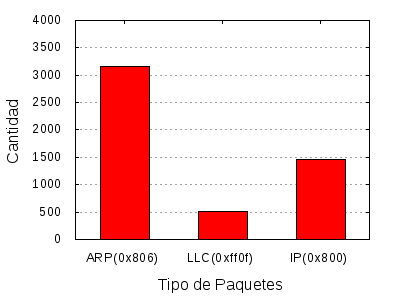
\includegraphics[width=0.45\textwidth]{figuras/experimento2-tipos-paquetes.png}
    \caption{Tipos de paquetes broadcast en el experimento 2.}\label{Tipos de paquetes}
\end{figure}

Como podemos observar en la figura \ref{Tipos de paquetes}, la mayor cantidad de paquetes son de tipo ARP. Podemos notar una pequeña cantidad de paquetes con tipo LLC (Logical Link Control). Éste es propio del estándar IEEE 802.2 que define el control de enlace l\'ogico para redes de \'area local en el modelo OSI. Estos dos tipos de paquetes son utilizados por protocolos de control y su funcionamiento requiere transmisión \textit{broadcast}. Lo llamativo aqu\'i es la gran cantidad de paquetes \textit{broadcast} de tipo IP.

Para mejor comprender esto, graficamos la cantidad de paquetes de este tipo enviados por IP de origen, como se puede ver en la figura \ref{Sources de paquetes IP broadcast}.

\begin{figure*}[ht]
    \centering
    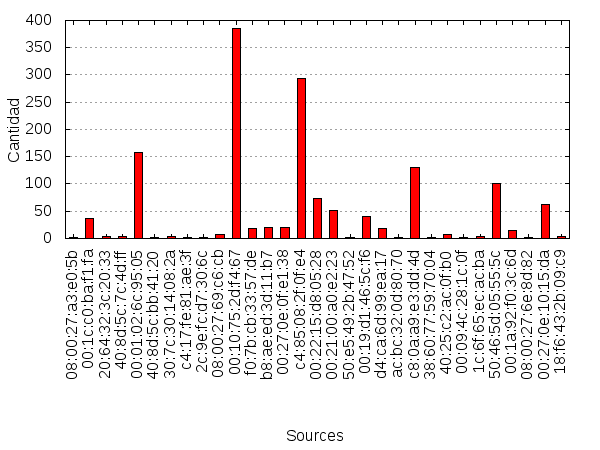
\includegraphics[scale=0.7]{figuras/experimento2-ips-origen.png}
    \caption{MAC addresses de los \textit{sources} de paquetes IP broadcast.}\label{Sources de paquetes IP broadcast}
\end{figure*}

Observemos los tres primeros \textit{sources} que sobresalen del resto en cuanto a cantidad de paquetes enviados. Éstos son los nodos cuyas MAC addresses son: 00:10:75:2d:f4:67 (386 paquetes), c4:85:08:2f:0f:e4 (294 paquetes) y 00:01:02:6c:95:05 (157 paquetes).
Analizando los paquetes de tipo IP que provenían de estos nodos en modo \textit{broadcast}, encontramos que emitían los siguientes mensajes:

\begin{itemize}
	\item 00:10:75:2d:f4:67	: Hello there. I am at 192.168.1.120. Time is 1474050708 and I am hungry.Hostname: backupdyd.seagateshare.com \\
		Notamos que se trata de un software de backup que podr\'ia estar notificando a todos los nodos sus datos para posteriores procesos.
            \item c4:85:08:2f:0f:e4	: De este \textit{source} no pudimos obtener mucha informaci\'on como para poder determinar el propósito de los paquetes \textit{broadcast}.
	\item 00:01:02:6c:95:0: 9016 3 ipp://192.168.1.150:631/printers/HP-LaserJet-P1006 "" "HP LaserJet P1006" "HP LaserJet P1006 Foomatic/foo2xqx (recommended)" job-shee    ts=none,none lease-duration=300 \\
		Se trata de mensajes emitidos por impresoras que eventualmente podr\'ian querer informar sus status a todos los nodos.
\end{itemize}

Por lo tanto, concluimos que se trata de paquetes de control, no de la red en sí misma, sino de protocolos propios de ciertos nodos.

\subsubsection{Estructura de la red en base a los paquetes ARP}

\par En la figura \ref{ARPlaburo} se puede ver el grafo de la red subyacente de mensajes ARP.

\begin{figure*}[ht]
    \centering
    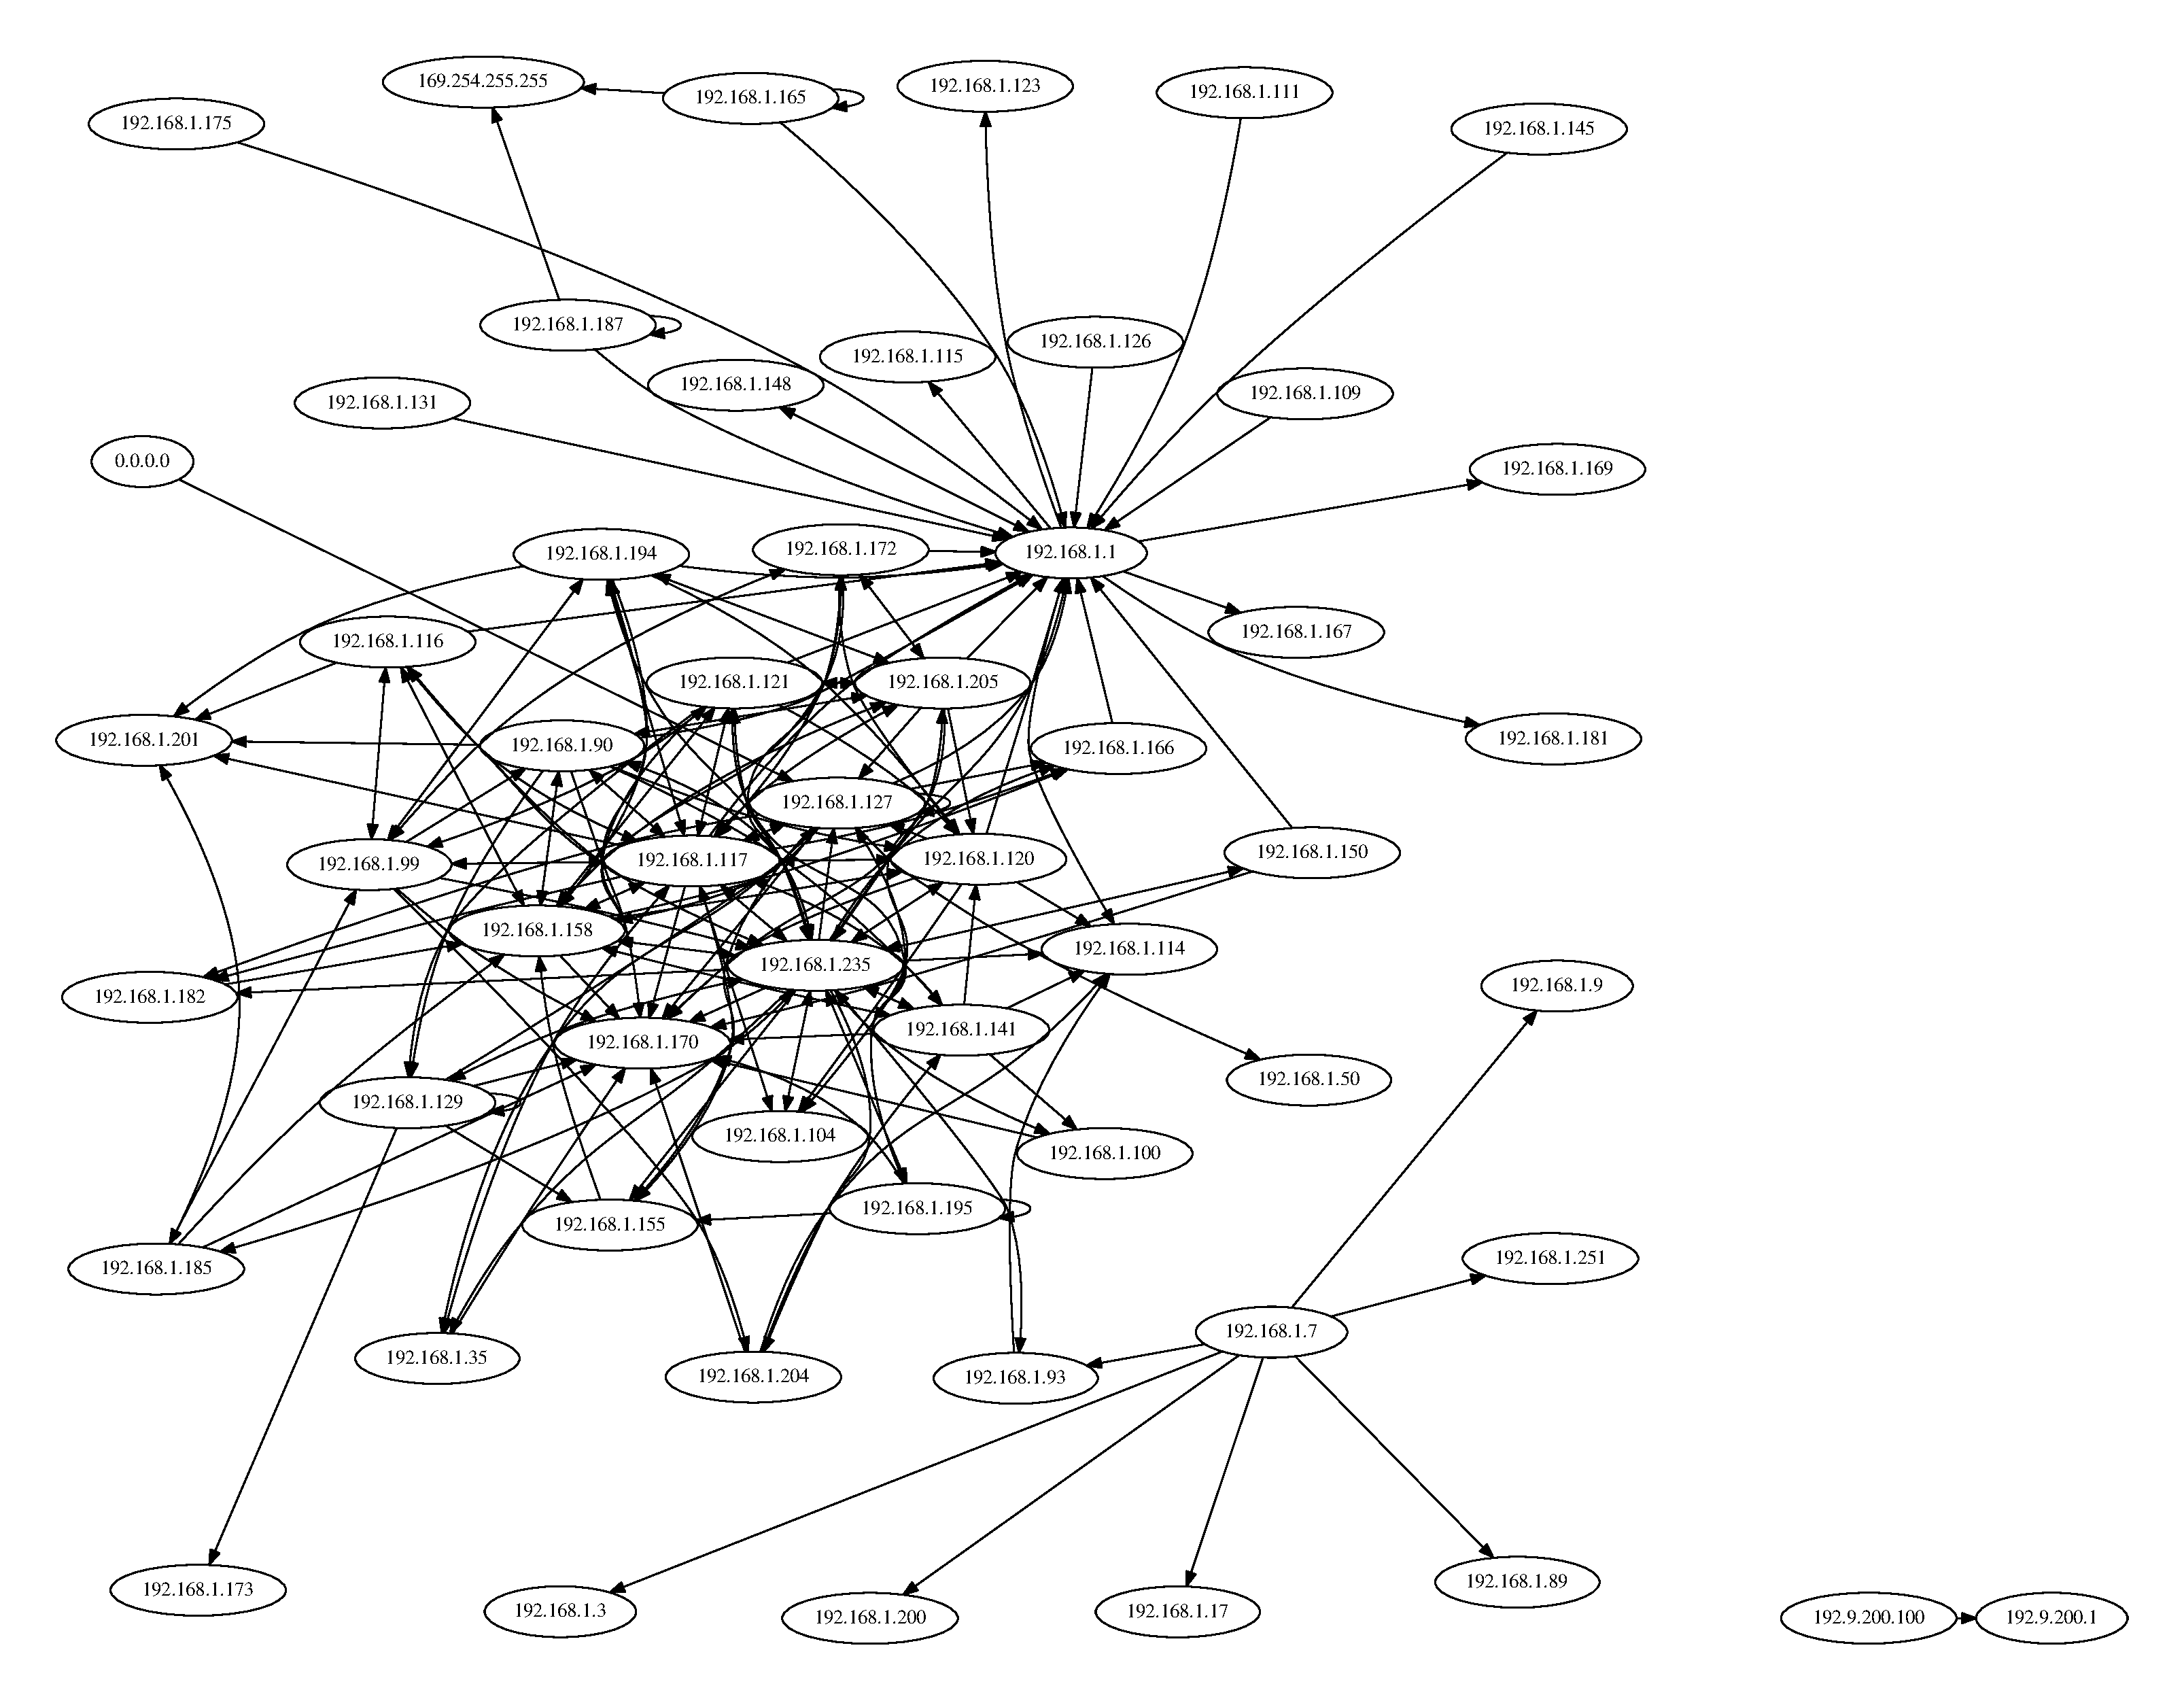
\includegraphics[width=0.9\textwidth]{figuras/laburo_grafo.pdf}
    \caption{Grafo de la red subyacente de mensajes ARP en el experimento 2.}\label{ARPlaburo}
\end{figure*}

\par Las direcciones IP de la red son de la forma 192.168.1.X, con ciertas excepciones: se observa la dirección 0.0.0.0 y la 169.254.255.255, ambas detalladas en el experimento previo; vemos dos nodos con las direcciones 192.9.200.100 y 192.9.200.1.
Adicionalmente, éstos son los únicos dos nodos que no están conectados al resto de la red.
Este comportamiento es anómalo, por lo que creemos que son IPs con un uso particular, específico a la red, ya que no parecen ser reservadas.

\par En el grafo se destaca claramente un nodo, el 192.168.1.1, cuyo comportamiento es consistente con lo esperado de un router\footnote{Es común que los routers ocupen la última o primera, como en este caso, dirección de la red.}.
Luego vemos un grupo de vertices con un muy alto grado de entrada y salida; sin embargo, no parecen actuar como Default Gateways.

\subsubsection{Fuente $S_1$}

\par En la tabla \ref{tab2SinRSinA} podemos ver la información de ciertos mensajes de la fuente $S_1$, sin paquetes repetidos y tomando sólo el \textit{Sender's Protocol Address} de los paquetes.

\par La entropía de la fuente es de 4.61 bits, siendo la máxima 32 bits. 

\begin{table}[t]
    \centering
    \begin{tabular}{ | c | c | c | l |}
        \hline
        Mensaje & Información [bits] & Distinguido?\\
        \hline
192.168.1.1 & 4.86 & No \\
\hline
192.168.1.194 & 4.50 & Sí \\
\hline
192.168.1.127 & 4.50 & Sí \\
\hline
192.168.1.90 & 4.34 & Sí \\
\hline
192.168.1.99 & 4.34 & Sí \\
\hline
192.168.1.121 & 4.34 & Sí \\
\hline
192.168.1.158 & 4.21 & Sí \\
\hline
192.168.1.205 & 4.08 & Sí \\
\hline
192.168.1.117 & 3.34 & Sí \\
\hline
192.168.1.235 & 2.96 & Sí \\
\hline
    \end{tabular} 
    \caption{Información de los nodos de la fuente $S_1$ en el experimento 2, sin tomar paquetes repetidos y considerando como mensaje la ocurrencia de una IP en el campo \textit{Sender's Protocol Address} de un paquete ARP \textit{who-has}.}
    \label{tab2SinRSinA}
\end{table} 

\par El resultado es el opuesto al esperado: los nodos distinguidos son los pertenecientes al grupo de vértices mencionado con alto grado de interconexión pero sin comportamiento de router, mientras que el nodo efectivamente identificado como Default Gateway no es distinguido.

\par En la tabla \ref{tab2A} podemos ver la información de ciertos mensajes de la fuente $S_1$, sin paquetes repetidos y tomando tanto el \textit{Sender's Protocol Address} como el \textit{Target Protocol Address} de los paquetes.

\begin{table}[t]
    \centering
    \begin{tabular}{ | c | c | c | l |}
        \hline
        Mensaje & Información [bits] & Distinguido?\\
\hline
192.168.1.194 & 4.86 & Sí \\
\hline
192.168.1.90 & 4.76 & Sí \\
\hline
192.168.1.99 & 4.67 & Sí \\
\hline
192.168.1.120 & 4.67 & Sí \\
\hline
192.168.1.121 & 4.67 & Sí \\
\hline
192.168.1.127 & 4.67 & Sí \\
\hline
192.168.1.170 & 4.50 & Sí \\
\hline
192.168.1.205 & 4.34 & Sí \\
\hline
192.168.1.158 & 4.08 & Sí \\
\hline
192.168.1.1 & 3.86 & Sí \\
\hline
192.168.1.117 & 3.58 & Sí \\
\hline
192.168.1.235 & 3.24 & Sí \\
\hline
    \end{tabular} 
    \caption{Información de los nodos de la fuente $S_1$ en el experimento 2, sin tomar paquetes repetidos y considerando como mensaje la ocurrencia de una IP tanto en el campo \textit{Sender's Protocol Address} como en el \textit{Target Protocol Address} de un paquete ARP \textit{who-has}.}
    \label{tab2A}
\end{table} 

\par La entropía de la fuente es de 4.93 bits, siendo la máxima 32 bits. 

\par Nuevamente se presentan los falsos positivos, pero el nodo que identificamos como router se considera ahora distinguido.


\newpage
\subsection{Experimento 3}
\par Realizamos este experimento sobre una red doméstica.

\subsubsection{Fuente $S$}

\par A continuación podemos ver la fuente $S$ propuesta, modelada con los resultados del experimento: \\

\begin{tabular}{ | c | c | c |}
    \hline
    Mensaje & Probabilidad & Información [bits] \\
    \hline
    \textit{Unicast} & 0.848 & 0.237 \\
    \hline
    \textit{Broadcast} & 0.152 & 2.720 \\
    \hline
\end{tabular} \\

\par Entropía de la fuente: 0.614 bits. Entropía máxima: 1 bit.

\par Observamos que la entropía de la fuente es menor que la máxima; las transmisiones \textit{unicast} son significativamente más probables que las \textit{broadcast}.
Esto nos indica que los protocolos de control tienen un bajo impacto en la \textit{performance} de la red.

\subsubsection{Estructura de la red en base a los paquetes ARP}

\par En la figura \ref{ARPcasa} se puede ver el grafo de la red subyacente de mensajes ARP.

\begin{figure*}[ht]
    \centering
    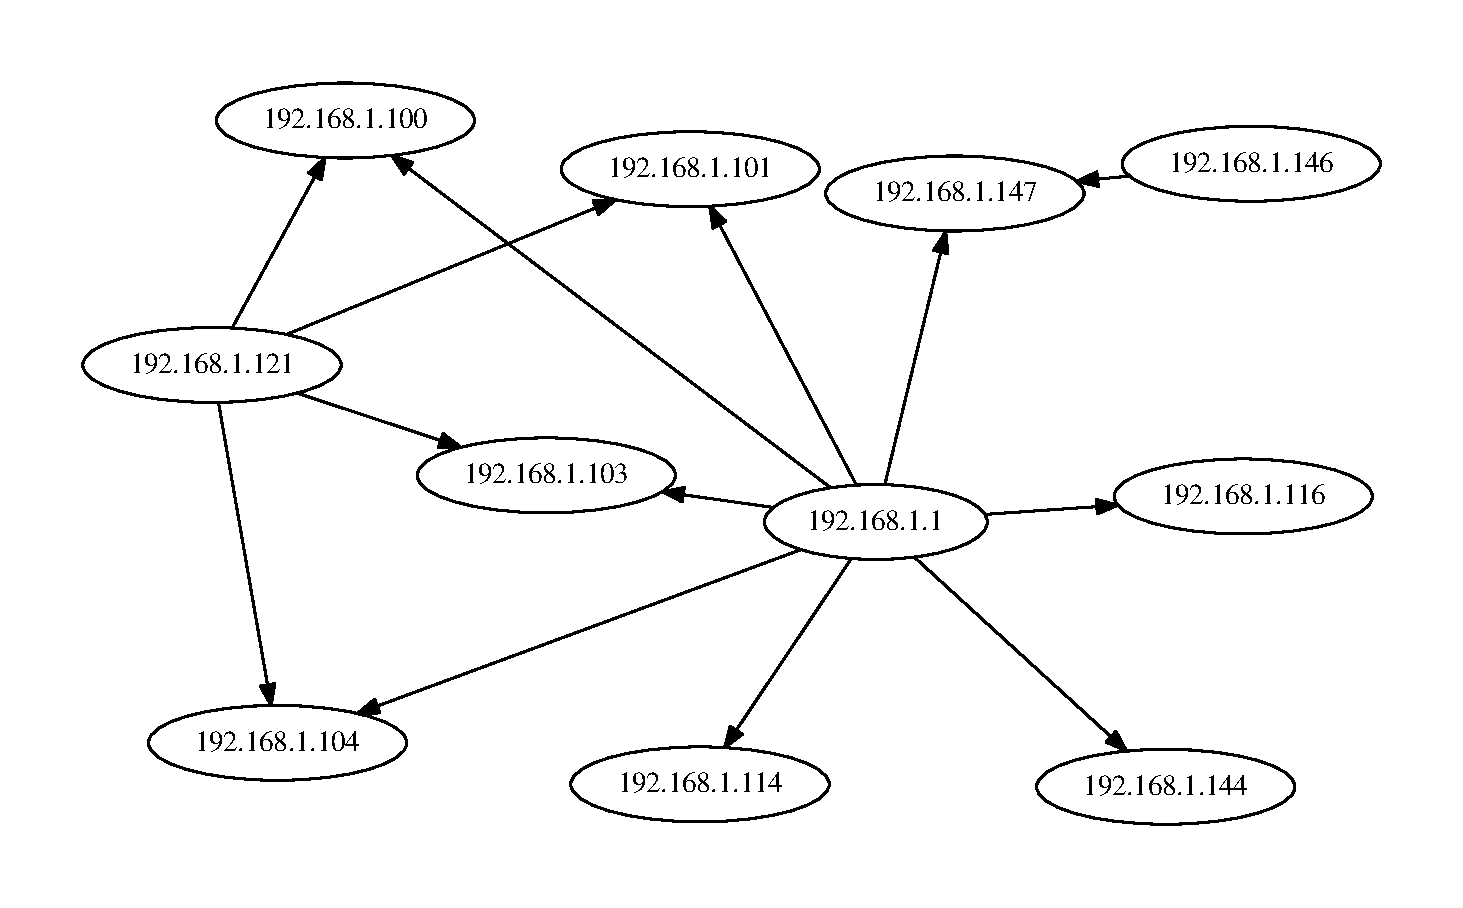
\includegraphics[width=0.9\textwidth]{figuras/casa_grafo.pdf}
    \caption{Grafo de la red subyacente de mensajes ARP en el experimento 3.}\label{ARPcasa}
\end{figure*}

\par Todas las direcciones IP de la red son de la forma 192.168.1.X.
Éstas son direcciones IP privadas\footnote{Todo el rango 192.168.0.0-192.168.255.255 es privado.}.

\par En el grafo se destaca claramente un nodo, el 192.168.1.1.
El vértice 192.169.1.121 también parece destacarse.
Una comparación entre las MAC addresses que acompañan a estas dos direcciones en los paquetes ARP y los diversos dispositivos de la red nos indicó que la 192.168.1.1 corresponde al router de la red, mientras que la 192.168.1.121, a la interfaz de una de las computadoras.

\subsubsection{Fuente $S_1$}

\par En la figura \ref{fig3SinRSinA} podemos ver la información de los mensajes de la fuente $S_1$, sin paquetes repetidos y tomando sólo el \textit{Sender's Protocol Address} de los paquetes.

\par La entropía de la fuente es de 1.24 bits, siendo la máxima 32 bits. 

\begin{figure}
    \centering
    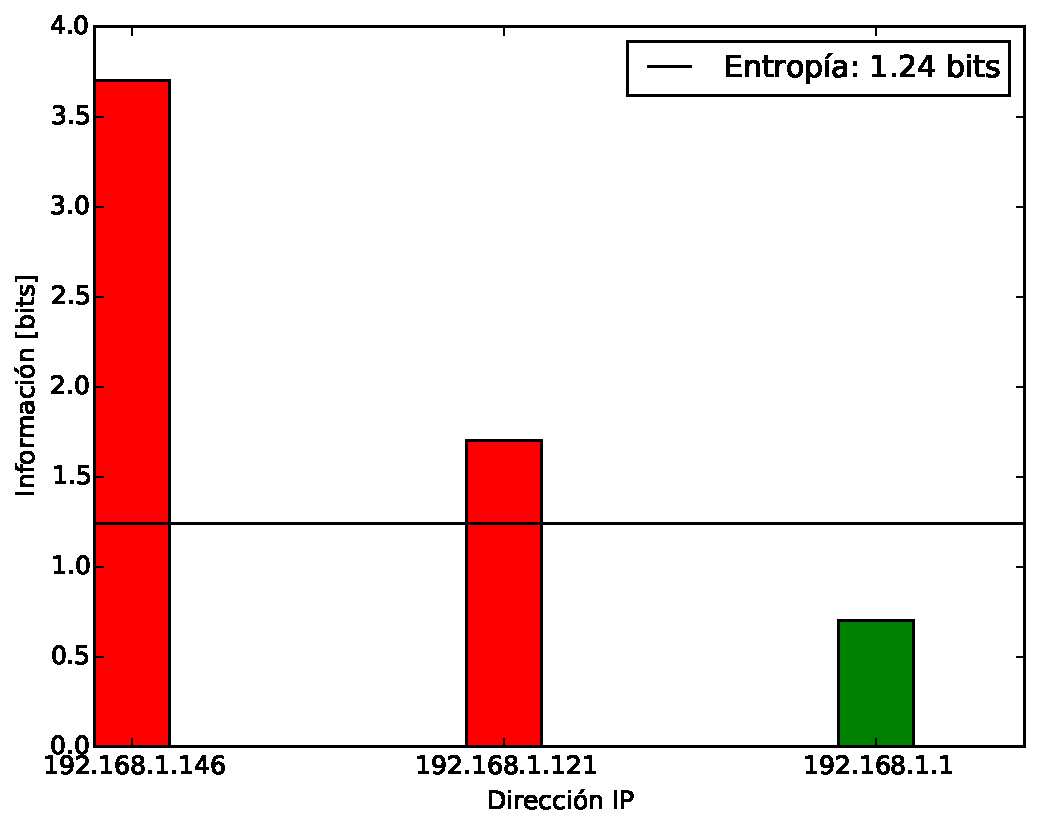
\includegraphics[width=0.45\textwidth]{figuras/casa_figura.pdf}
    \caption{Información de los nodos de la fuente $S_1$ en el experimento 3, sin tomar paquetes repetidos y considerando como mensaje la ocurrencia de una IP en el campo \textit{Sender's Protocol Address} de un paquete ARP \textit{who-has}.}
    \label{fig3SinRSinA}
\end{figure}

\par La fuente clasifica exactamente de la forma deseada: el único nodo distinguido es el correspondiente al router.

\par En la figura \ref{fig3A} podemos ver la información de los mensajes de la fuente $S_1$, sin paquetes repetidos y tomando tanto el campo \textit{Sender's Protocol Address} como el \textit{Target Protocol Address} de los paquetes.

\par La entropía de la fuente es de 3.09 bits, siendo la máxima 32 bits. 

\begin{figure}
    \centering
    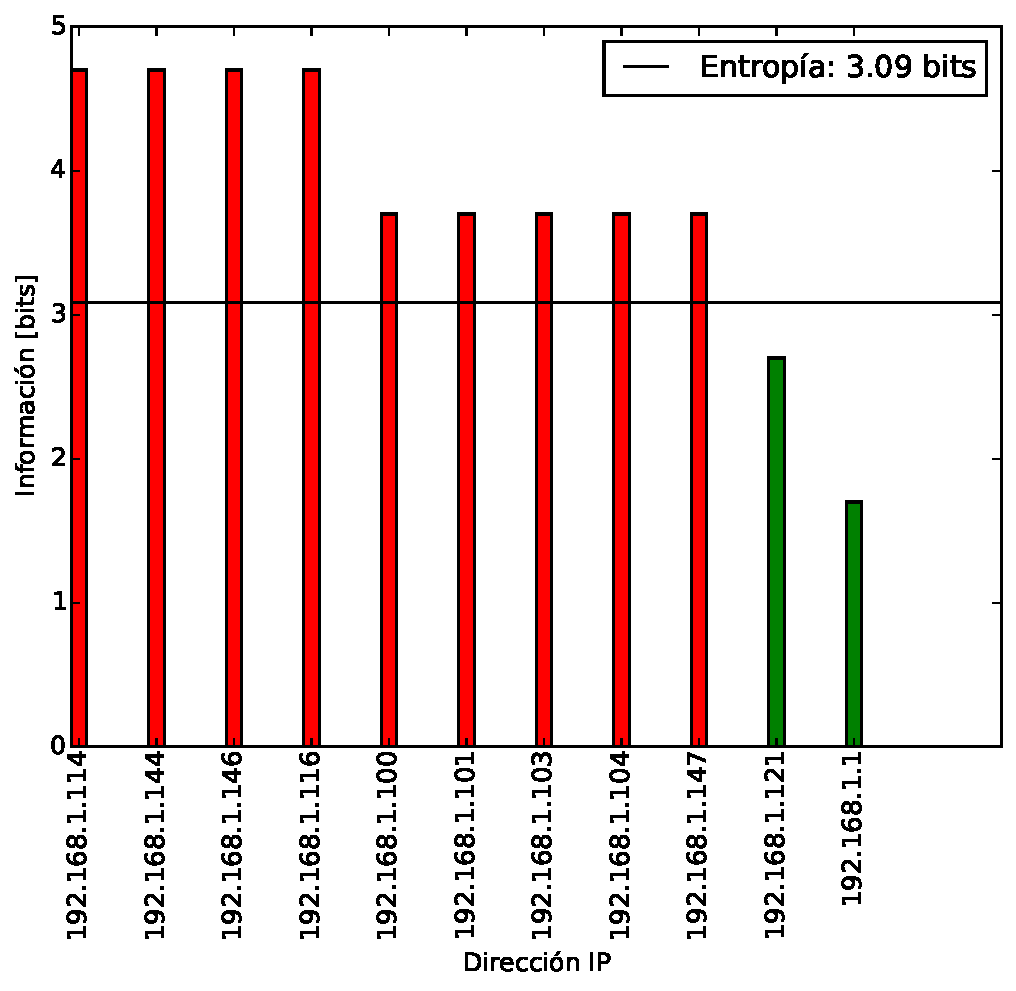
\includegraphics[width=0.45\textwidth]{figuras/casa_figura_ambos.pdf}
    \caption{Información de los nodos de la fuente $S_1$ en el experimento 3, sin tomar paquetes repetidos y considerando como mensaje la ocurrencia de una IP tanto en el campo \textit{Sender's Protocol Address} como en el \textit{Target Protocol Address} de un paquete ARP \textit{who-has}.}
    \label{fig3A}
\end{figure}

\par Al igual que en los otros experimentos, la entropía es mayor al considerar esta fuente.

\par Se presenta un falso negativo, el previamente mencionado nodo 192.168.1.121.
Este resultado es interesante ya que éste actúa exclusivamente como emisor, por lo que la cantidad de veces que aparece en ambas fuentes es igual; la mayor entropía de esta fuente lleva a que sea clasificado como vértice distinguido.
